 \documentclass{sig-alternate}
\usepackage{hyperref}

\begin{document}
%\conferenceinfo{WWW}{'15 Florence, Italy}

\title{The Open Access Academia Corpus}

\numberofauthors{1}
\author{
\alignauthor
Andrew Yates, Rajiv Ramnath, Shashank Agarwal\\
\affaddr{Department of Computer Science and Engineering}\\
\affaddr{The Ohio State University}\\
\email{\{yates,ramnath,agarwash\}@cse.ohio-state.edu}
}

\maketitle
\begin{abstract}
The growth of open access (OA) academic publication worldwide
challenges libraries and academics about how to organize, rank, and
include new work in library catalogs. However, systematic evaluation
of trends in cross-disciplinary open access publication is hindered by
fragmentation of sources and inconsistent presentation of content. To
facilitate research in this space, we have compiled the holdings of
the three largest directories of open access academic publications:
Directory of Open Access Journals (DOAJ), PubMed Central Open Access
(PMC OA), and ArXiv. We standardize record format to support
cross-source comparison, and we apply a variety of heuristics and
external sources to improve record quality. We publish this corpus of
2,788,559 documents as a freely available resource at
\url{http://goo.gl/KOlgVX}. %% oaacademia.org?

\end{abstract}

% A category with the (minimum) three required fields
\category{A.2}{Reference (e.g., dictionaries, encyclopedias, glossaries)}{}
%A category including the fourth, optional field follows...
\category{I.7.0}{Document And Text Processing}{General}

\keywords{Open access; Compilation; Document archive}

\section{Introduction}

Open access academic publication refers to unrestricted access to
scholarly work hosted on the web. Interest in open access publication
as a trend in academia ranges from the political\cite{Shavell2010} to
the philosophical\cite{Willinsky2006} to improving scientific access
internationally\cite{Gasparyan2013} to increasing scientific impact as
measured by views\cite{Bollen2009}, citations\cite{Davis2011,
  Hitchcock2013, Lawrence2001} and impact factor\cite{Giglia2010,
  Brink2013}. However, open access is perhaps best understood as an
aspect of the general trends associated with the Internet of the last
decade: accelerating production of media, virtually free, immediate,
and omnipresent distribution, and the easy of publishing by anybody
worldwide. While the prevalence and importance of open access
publication has been well researched\cite{Bjork2010, Bjork2013}, here we
address the challenges and opportunities of open access publishing as
they relate to computer science research.

On one hand, open access publishing makes complete academic
publications available in a free and easy to access format over the
Internet, enabling researchers to find and study trends in the corpus
of all academia. Also importantly, open access publications are not
only technically available, but also legally available, and are
released under licenses permitting such research. On the other hand,
the easing of barriers to publication and the acceleration of content
production circumvent traditions and institutions of scholarly
reputability like university libraries and print journals, leading to
the familiar problems of other electronic media like floods of
fraudulent or low quality content \cite{Beall2012} and difficulties in
discovering and organizing new publications.

To mitigate these problems, much work has been done to organize open
access publications into online directories like the Directory of Open
Access Journals (DOAJ), PubMed Central Open Access (PMC OA) and ArXiv
and online search tools like Google Scholar and CiteSeerX
\cite{Giles1998}. These resources have been great boons to both
academics and to computer scientists today and in the past. However,
proprietary tools like Google Scholar forbid batch processing of their
indexes, and tools like CiteSeerX and DBLP\cite{DBLP} are limited to single domains like
computer science. To explore the domain of all open access science, an
open compilation of open access directories across disciplines is
needed to standardize record format, combine cross-referenced entries,
and ameliorate the myriad of data quality issues known to affect
directories of academic work. \cite{Beall2006}\cite{Ley2006}.

We create such a compilation, The Open Access Academia Corpus (OAAC),
and publish it at \url{http://goo.gl/KOlgVX}. We
were motivated to create this compilation for use in our own computer
science research in natural language processing and document
clustering, and we hope that other academics will find it useful as
well. To our knowledge, this is the largest, most complete corpus of
open access academic research freely available on the web. The main
advantage of using OAAC in computer science research is that it
combines a wide variety of disciplines, topics, and writing styles
while maintaining the high standards of rigor, substance, structure,
and affiliations required in academic publishing. This makes OAAC
particularly useful in research related to topical content analysis on
a large scale. 

\section{Sources}
OAAC is a standardized and computationally curated compilation of
other authoritative directory resources. To create OAAC, we compile
the complete contents of the three largest general open access
directories of open access academic publications as of March 2014. We
download record metadata in bulk from the services provided by these
repositories.

\subsection{Primary Sources}

\textbf{Directory of Open Access Journals (DOAJ)} aims to index all
open access peer-reviewed journals in all disciplines worldwide. At
this time, it indexes 9,713 Journals and 1,502,700 articles from 133
countries.\cite{Morrison2008} \\URL: \url{doaj.org}

\textbf{ArXiv} (pronounced ``archive'') is a repository of
929,442 open access academic preprints (author-published) of physics,
mathematics, computer science, and other quantitative fields. Many of
these preprints are later published in other journals. \\URL: \url{arxiv.org}

\textbf{PubMed Central Open Access Subset (PMC OA)} makes available a
subset of 774,993 biomedical science publications in PubMed Central
that were released under permissive licenses. \\URL: \url{ncbi.nlm.nih.gov/pmc/tools/openftlist}

\subsection{Supplementary Sources}
We also supplement and extend primary source record entries using the
following resources:

\textbf{Digital Object Identifier System (DOI)}
assigns and enforces persistent unique identification of objects of
any type, in particular, of academic publications. As part of the
service, dx.doi.org stores some metadata about objects in the DOI
system including author names, journal name, publisher name, and
related ISSNs (International Standard Serial Number). When DOIs are
included in a record, we query dx.doi.org to confirm and supplement
the record. \\URL: \url{dx.doi.org}

\textbf{JournalTOC (Journal Tables of Contents)}
       is the largest, free collection of
       scholarly journals, which lists 24,229 journals by ISSN. When
       ISSNs are included in a record, we query JournalTOC to confirm
       the journal name and publisher. \\URL: \url{journaltocs.ac.uk}

\section{Compilation}

\begin{figure}[ht]
\centering
  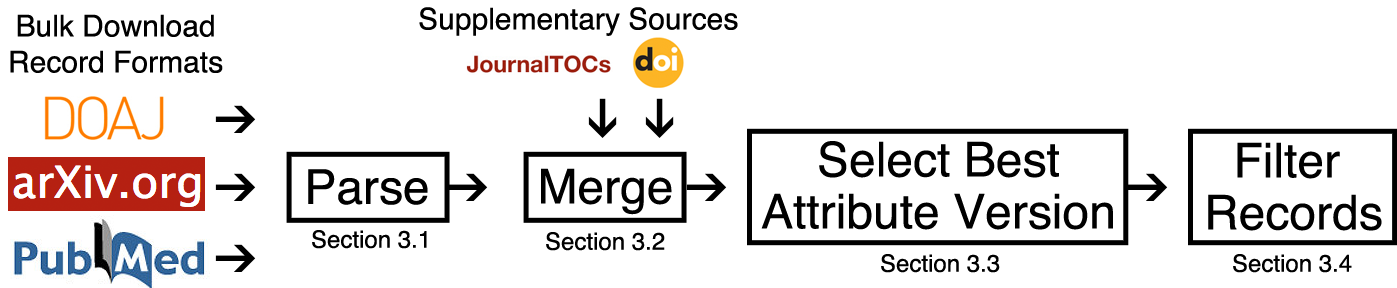
\includegraphics[width=\linewidth]{figures/DBWorkflow}
  \caption{\label{fig:workflow} Corpus Generation Workflow}
\end{figure}

\subsection{Parse Source Record Format}
Over the course of March 2014, we downloaded the entire directories of
DOAJ (1,502,700 records), arXiv (929,442 records) and the PubMed
Central OA subset (774,993 records) using each services’ bulk download
tools for a total of 3,207,135 records. Each of these tools produced a
variety of different files in a variety of formats. We wrote custom
parsers for each different file type to standardize each source record
as a Python dictionary object of Unicode strings. Cleaning records
included decoding XML, HTML, and LaTeX encoded character sequences to
Unicode, collapsing whitespace strings to single spaces, stripping
spurious presentation markup and whitespace padding, and representing
author names in a standard format of given names first, surname last,
and initials followed by a period. In the case of arXiv, we also
converted arXiv, ACM (American Computing Machinery classification
system, \url{acm.org/about/class/ccs98-html}), and MSC (Mathematics
Subject Classification) subject tags to their plain text mappings as
additional tags. In the case of DOAJ, we did not include DOAJ-suggested
categories as tags.

\subsection{Merge Duplicates}

\begin{figure}[ht]
\centering
  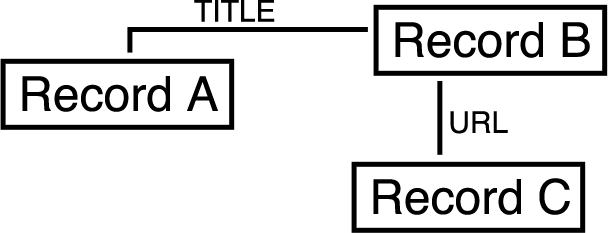
\includegraphics[width=0.7\linewidth]{figures/equiv_set}
  \caption{\label{fig:graph} Records A, B, and C are aggregated to form a unique merged record.}
\end{figure}

To merge together duplicate records, we created record equivalence
classes linked by URLs, title, or DOI. One could think of this process
like finding connected components in a graph where nodes are records,
edges are a shared URL, title, or DOI, and each connected component is
a unique merged record; see Figure \ref{fig:graph}. Connected
components can be computed in $O(E+V)$ time.\cite{Cormen2009} For each
merged record, we also added any supplementary record information as
linked by DOI or ISSN. The resulting merged record is a set of
attributes where the value of each attribute is list of values from
all included sources. 2,842,026 unique records remain after merging.

\subsection{Select Best Attribute Version}
We select the best form of each attribute by a variety of heuristics
that differ slightly for each attribute type. In general, we convert
all attributes to strings and select most frequent value first and
then by the longest string with the largest upper-lower case
entropy. For URL, we preferentially select the URL that is not at a
known directory domain and that has either a .pdf or .html
extension. For author list, we prefer the author list as provided by a
source in PubMed, arXiv, dx.doi.org, and DOAJ in decreasing order of
preference. We also examine all other author lists and the abstract
for any matches of surnames adjacent to any names that could expand
any initials in the preferred author list. In all cases, we keep any
unselected alternate forms of any duplicate attributes with the record
in the special \textsl{alt} attribute; see Appendix. We do not mirror full
document texts; instead we assume that URLs served as proxies to
copies of the full document text online.

\subsection{Filter Records}
We define a valid record to have a title, at least one author, at
least one URL and at most one DOI. Further, we require documents to
have unique titles and URLs as a standard of quality control. To
support duplicate records while removing spurious records with
non-unique titles like ``Errata'' or non-unique URLs pointing to
journal homepages, we limited the number of primary source records in
a single merged record to 4. We remove any record that did not meet
these criteria. After filtering, 2,788,559 valid records (98.1\%)
remain. Finally, we assign each record a unique alphanumeric ID. We
publish this filtered collection of valid, merged, unique records as
the ``FULL'' set.

\subsection{Identifier Validation}

We validate ISSN, DOI, and URL article identifiers using standard
techniques. For DOIs, we check well-formed identifiers for usage on
Google Scholar \cite{scholar2014} and crossref.org. For URLs, we test reachability using
an ordinary HTTP request. We mark records returning HTTP code 200 as
valid.

\section{Corpus}

We publish our compiled corpus and related files at
\url{http://goo.gl/KOlgVX} for free anonymous downloading over the
Internet. For ease of use, each line is in a self-contained Python
string format (``pickle'' format), one line per record. This is so
that the file may be processed per line without having to read the
entire file into memory, to avoid character encoding errors, and to
facilitate the use of ordinary unix tools like grep. See Figure
\ref{fig:code} for a code usage example in Python. We also have
shuffled the line order from the processing order so that any block of
lines is a valid random sample of the entire corpus.

\begin{figure}[ht]
\begin{verbatim}
for line in open(FILE_NAME):
  record = eval(line) 
\end{verbatim}
\caption{\label{fig:code} Example Python code for on-line record handling from file.}
\end{figure}

\subsection{Corpus Statistics}
The compiled corpus has a wide coverage of unique journals, authors,
and languages; see the following list. Of records unassociated with a
journal, most (95.5\%) are arXiv preprints without publication records
and are presumably unpublished. We flag unpublished articles for easy
filtering as they may indicate low quality records; see Appendix.

\begin{figure}[ht]
\centering
  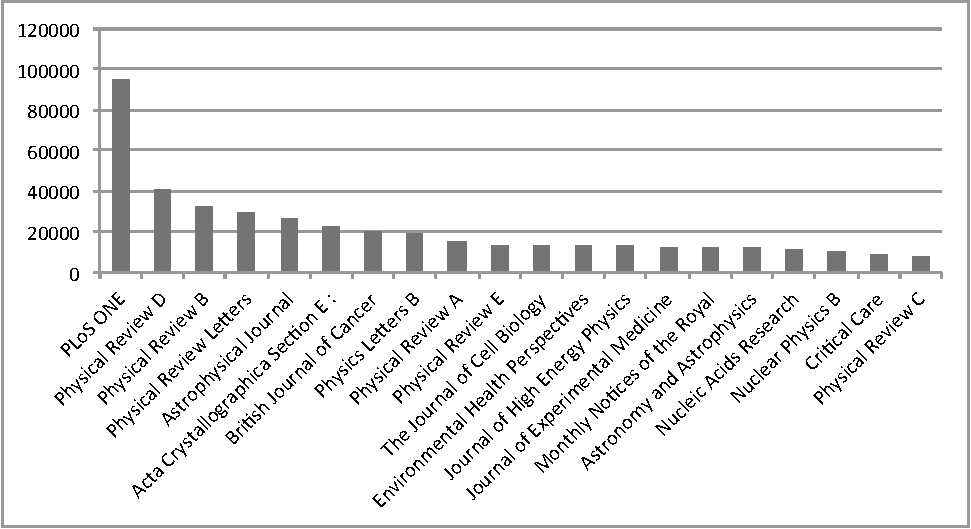
\includegraphics[width=\linewidth]{figures/journals}
  \caption{\label{fig:journals} Top 20 Journals by Document Count. 529,435 documents have no journal.}
\end{figure}

\begin{figure}[ht]
\centering
  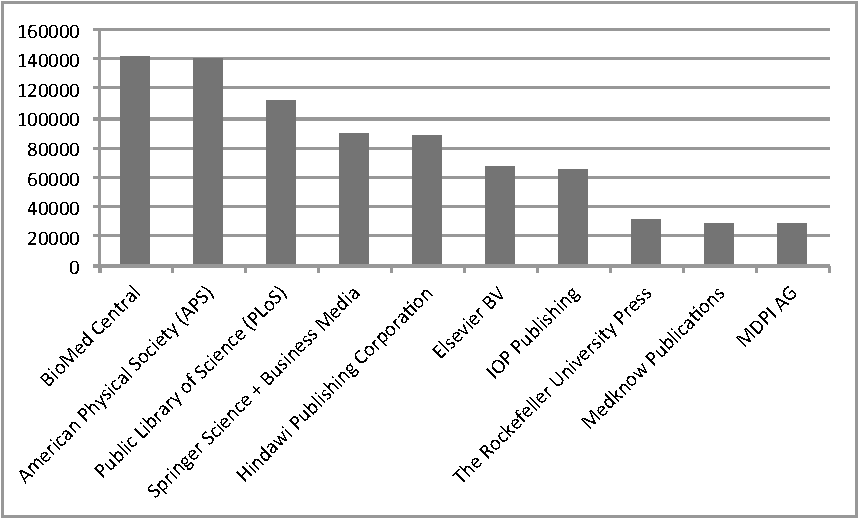
\includegraphics[width=\linewidth]{figures/publishers}
  \caption{\label{fig:publishers} Top 10 Publishers by Document Count. 530,449 documents have no publisher.}
\end{figure}

\begin{description} \itemsep1pt
  \item[Journals] 13,197
  \item[Publishers] 5,187
  \item[Authors] 3,916,477
  \item[Reported Languages] 70
  \item[Has DOI] 1,461,082 (53.3\%)
  \item[Has Abstract] 2,534,770 (90.9\%)
  \item[Has Tags (Keywords)] 1,966,508 (70.5\%)
  \item[Associated with Journal] 2,270,960 (81.4\%)
  
\end{description}

Not surprisingly, as shown in Figure \ref{fig:publishers}, BioMed
Central and the American Physical Society are the top two publishers
as these two publishers are highly represented in PubMed Central OA
and ArXiv respectively. The Public Library of Science (PLoS), perhaps
one of the most well-known Open Access academic publishers, the third
most common publisher in OAAC; however, PLoS ONE is by far the most 
frequent journal as shown in Figure \ref{fig:journals}.

\begin{figure}[ht]
\centering
  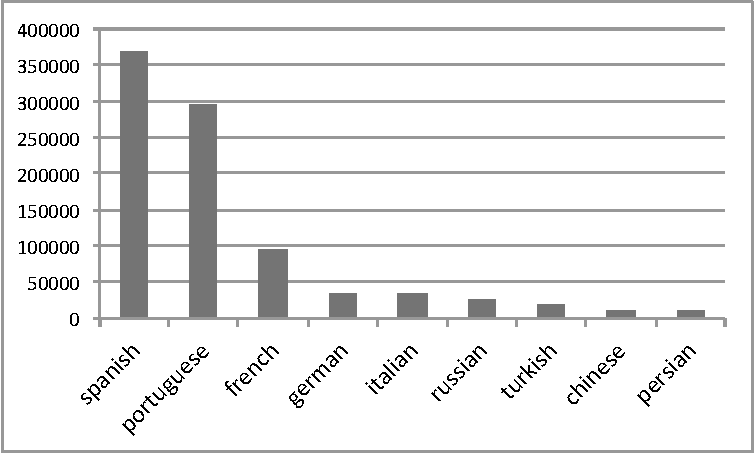
\includegraphics[width=\linewidth]{figures/language}
  \caption{\label{fig:languages} Top 10 Declared Languages excluding English (1,441,076) and None (1,112,098).}
\end{figure}

\subsection{English Language}
The language of most records were either labeled as English or left
unlabeled with the assumption that they were English in the source
directories; see Figure \ref{fig:languages}.  However, we found that
the reported language, if any, frequently mismatched the actual
language of the record. In DOAJ records particularly, languages were
frequently mixed languages together within the same record and even
within the same block of text. Also, sometimes values contained mostly
XML markup and little or no plain text. To mitigate these issues, we
used English language spellcheck software to identify records with a
majority of ordinary English words. We provide this subset of
2,054,452 documents (73.7\% or FULL) as a separate corpus (ENGLISH).

\subsection{Standardized Random Samples}
A corpus of over two million records can be unwieldy and a large file
to store (uncompressed, 6.2GB FULL, 4.5G ENGLISH). To support more
tractable data science experiments while providing standardized
benchmark datasets, we have pre-compiled five files of 1,000 randomly
selected records each (RANDOM\_1K\_1 through RANDOM\_1K\_5).

\subsection{Unmerged Parsed Records}
We also provide the set of unmerged parsed records per merged record
as produced in Section 3.1 (PARSED). These records are not
standardized, and their format depends on from which primary source
they derive. However, they may contain additional information like
author affiliation that has been discarded while merging.

\section{Web Service}

Going through millions of lines to find specific article can be a daunting task,
so to simplify access to specific articles from the OAAC we created a web service. 

The WebService follows REST protocol and returns a json object on a valid request.
The Webservice is hosted at \url{http://oaacademia.org/rest} and is built with `php` and uses
mysql (AWS RDS) as the backend. 

The full documentation is available at \url{http://oaacademia.org/rest}. Some methods are also
explained in Appendix.

\subsection{Example usage} 
A GET request to get a list of articles offset at `start` and limited by `count`. 
URL: \url{http://oaacademia.org/rest/get_articles/start/count}. This 
will return a JSON object with the articles.
Example: \url{http://oaacademia.org/rest/get_articles/0/100}, returns the first 100 articles 
from the corpus.

To get a specific article by the record id as given in the OAAC, a GET request is made to
 \url{http://oaacademia.org/rest/get_article_by_alternate_id/id}
 
 Example: \url{http://oaacademia.org/rest/get_article_by_alternate_id/G22L1FR6W5CTSSOA}.
 The request returns a JSON object with id, title, abstract, url, journal, publisher etc of the article 
 requested.


\section{Discussion}

OAAC contains a large collection of Open Access academic publications
from wide variety of disciplines.  As a corpus of text samples, it is
particularly useful in computer science research related to content
analysis on the web because it is diverse in document topics yet
relatively consistent in quality, sophistication, and
format. Nevertheless, many opportunities for future work on OAAC
exist. First, OAAC aggregates the records of several other
directories, thus the quality and completeness of OAAC records must
depend on the quality and completeness of these directories. While
compiling these directories produce form a ``wisdom of crowds''
aggregated record corpus of sorts, there is much potential for
processing the full publication texts themselves, which we do not
do. Second, we have only produced a snapshot of OA Academia at the
time we compiled OAAC (Spring 2014). Ideally, new publications would
be added to OAAC as they are published automatically. Finally, we
produced OAAC primarily for computer science researchers who would be
most interested in downloading the corpus and processing it
themselves. However, other tools could be built around OAAC like a
database-driven web interface to encourage usage to a wider audience
and support features like search and database queries.

%\end{document}  % This is where a 'short' article might terminate

%ACKNOWLEDGMENTS are optional
\section{Acknowledgments}

Supported by Amazon AWS in Education Research Grant Award and by a
grant from OCLC. Shashank Agarwal helped with downloading DOAJ
records.


%
% The following two commands are all you need in the
% initial runs of your .tex file to
% produce the bibliography for the citations in your paper.
\bibliographystyle{abbrv}
\bibliography{open-access}  % sigproc.bib is the name of the Bibliography in this case
% You must have a proper ".bib" file
%  and remember to run:
% latex bibtex latex latex
% to resolve all references
%
% ACM needs 'a single self-contained file'!
%
%APPENDICES are optional
%\balancecolumns
\appendix
%Appendix A
\section{Description of Record Attributes}
Each record in OAAC is a Python dictionary of key, value pairs. Any
unknown attribute has the value \textsl{None}. We list all keys here
with a brief description of the values that may be assigned to each
key.

\subsection{Document}
\begin{description} \itemsep1pt
  \item[id] An 16 alphanumeric ID that uniquely identifies the record in the corpus
  \item[title] Document title
  \item[authors] A list of the document authors in published order. Each name is a single string with given names first and in order and then surname.
  \item[abstract] The document abstract.
  \item[url] The web link to the document��'s full text.
  \item[tags] A list of any author or journal provided keywords, tags, or categories.
  \item[url\_valid] A boolean flag indicating if the url returned a valid response when called.
  \item[record\_valid] A boolean flag indicating if the record is valid or not, if the url is invalid the record is marked as invalid.
  \item[last\_updated] The date in format DD-MM-YYYY TMZ, indicating when was the record last validated and updated.
  \item[version] The version number shows in which revision of the OAAC was the record modified or added.


\end{description}

\subsection{Publication}
\begin{description} \itemsep1pt
  \item[journal] Full name of journal in which the document is published.
  \item[publisher] Full name of the publisher that published the document
  \item[doi] Digital Object Identifier, a unique ID assigned to
    published works by the International DOI Foundation (IDF). See
    doi.org for more information. DOIs refer to individual
    documents. DOIs begin with ``10.''
  \item[issns] Set of International Standard Serial Numbers (ISSNs)
    associated with the document. ISSNs refer to journals and
    periodical publications rather than individual documents. ISSNs
    are in the form of the regular expression:
   \begin{verbatim}\d{4}\-\d{3}[\dX]\end{verbatim}
  \item[year] earliest recorded publication year
  \item[page] page number in publication
  \item[issue] issue of publication
  \item[volume] volume of publication
  \item[language] list of languages claimed by the journal and the
    document author. Note that the actual language of the record and
    its associated document may differ.
\end{description}

\subsection{Meta}
\begin{description}\itemsep1pt
  \item[referenced] A dictionary of references to supplementary records used to create the merged record. 
    \begin{description}\itemsep1pt
      \item[doaj\_journal]: DOAJ Journal meta record; see \url{doaj.org/faq#metadata}
      \item[issn]: JournalTOC ISSN record
      \item[doi]: \url{dx.doi.org} DOI record
    \end{description}
  \item[merged\_info] Set of tuples of the parsed records included in this merged record. In each tuple, the letter indicates the source, while the number indicates the record number from that parsed source file. Letter Codes: A: ArXiv, O: OCLC-provided subset, D: DOAJ, P: PubMed.
  \item[spellcheck] A dictionary of spell check results for the title, abstract, and tags attributes.
    \begin{description}\itemsep1pt
      \item[eng\_pct]: fraction of words recognized by an English spell checking program
      \item[xml\_pct]: fraction of common XML characters like <, >, and \&
    \end{description}
  \item[accept\_text] Indicates whether the record passed the
    ``sufficient English'' test field: title, abstract (abstr), and
    tags. \textsl{None} indicates a failure of the entire record to
    pass the ``sufficient English'' test. Note that the record as a
    whole can pass the test despite that some of the fields have
    failed the test.
  \item[alts] A dictionary of attribute key names to a list of
    alternate values for that attribute. We save these alternate
    values rather than discarding them after selection of the best
    attribute version as described in Section 3.3.
  \item[is\_published] A boolean flag indicating whether the document record has a known journal or publisher associated with it.
\end{description}

\section{Consuming the WebService}
The WebService can be used to get data from the OAAC for specific articles or to access all articles.
The following are some methods implemented in the Web-service.

\subsection{GET /get\_articles/}
Get a list of all articles starting from "start" location and limited by "count" If the "start" is not given, the API by default returns the first 20 articles.
\begin{description} \itemsep1pt
  \item[url] \url{http://open-academia.org/rest/get_articles/start/count}
  \item[start] (int) The offset from start of index
  \item[count] (int) The number of records to return
\end{description}

\subsection{GET /get\_article\_by\_alternate\_id/}
Get article details for the specified "alternate\_id"
\begin{description} \itemsep1pt
  \item[url] \url{http://open-academia.org/rest/get\_article\_by\_alternate\_id//{alternate\_id}}
  \item[alternate\_id] (varchar) The unique id of article as in OAAC 
\end{description}

\subsection{GET /get\_article\_by\_id}
Get article details for the specified "article\_id"
\begin{description} \itemsep1pt
  \item[url] \url{http://open-academia.org/rest/get\_article\_by\_id/{article\_id}}
  \item[article\_id] (int) A Unique ID assigned to every article by Web-Service
\end{description}

\subsection{GET /get\_authors}
Get a list of authors associated with the specified "article\_id"
\begin{description} \itemsep1pt
  \item[url] \url{http://open-academia.org/rest/get\_authors/{article\_id}}
  \item[article\_id] (int) A Unique ID assigned to every article by Web-Service
\end{description}

\subsection{GET /get\_journal}
Get journal name associated with the specified "article\_id"
\begin{description} \itemsep1pt
  \item[url] \url{http://open-academia.org/rest/get\_journal/{article\_id}}
  \item[article\_id] (int) A Unique ID assigned to every article by Web-Service
\end{description}

\subsection{GET /get\_tags}
Get tag names associated with the specified "article\_id"
\begin{description} \itemsep1pt
  \item[url] \url{http://open-academia.org/rest/get\_tags/{article\_id}}
  \item[article\_id] (int) A Unique ID assigned to every article by Web-Service
\end{description}











\end{document}
